\begin{sidewaysfigure}[htbp]
\centering 
  \subfloat[\acs{mus} = 0.1, \acs{mur} = 0.4, $v_{inlet}$ = 100 m/s .]
  {
	  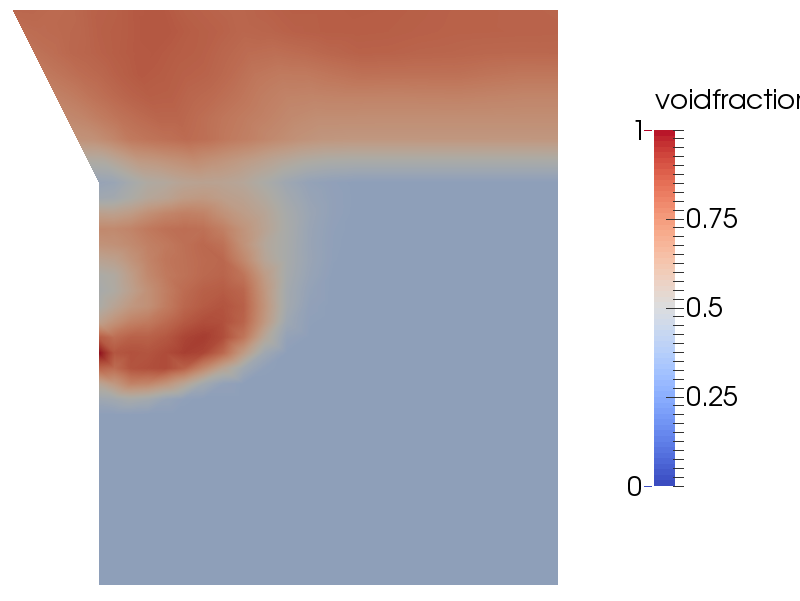
\includegraphics[width=.3\columnwidth]{images/235vf_average_lf}
	  \label{fig:235vf_average_lf}
  }
  \quad
    \subfloat[\acs{mus} = 0.5, \acs{mur} = 0.4, $v_{inlet}$ = 100 m/s .]
    {
	  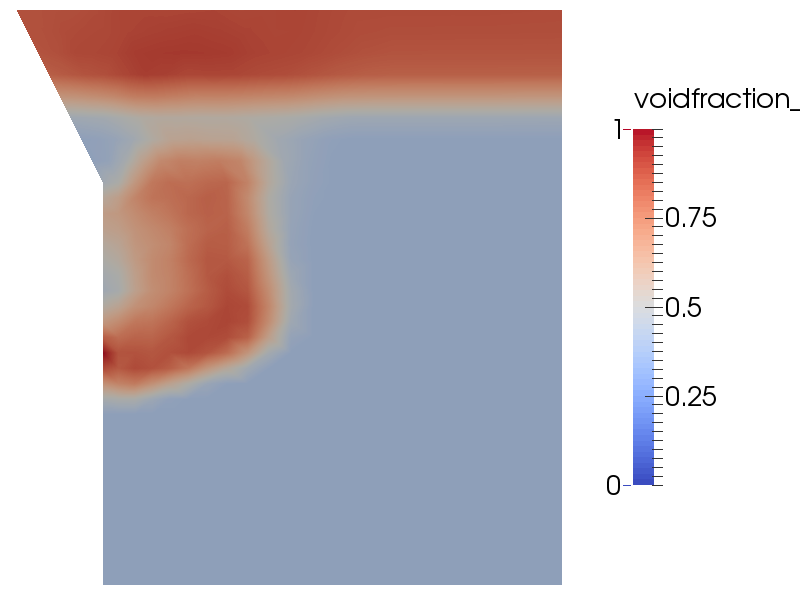
\includegraphics[width=.3\columnwidth]{images/254vf_average_mf}
	  \label{fig:254vf_average_mf}
  }
  \quad
    \subfloat[\acs{mus} = 0.9, \acs{mur} = 0.4, $v_{inlet}$ = 100 m/s .]
    {
	  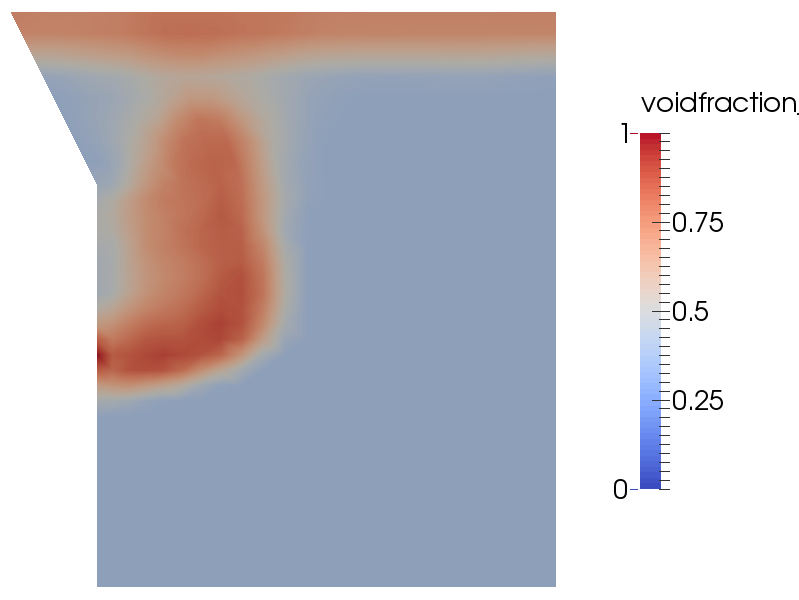
\includegraphics[width=.3\columnwidth]{images/234vf_average_hf}
	  \label{fig:234vf_average_hf}
  }
  \\
  \subfloat[\acs{mus} = 0.1, \acs{mur} = 0.4, $v_{inlet}$ = 200 m/s .]
  {
	  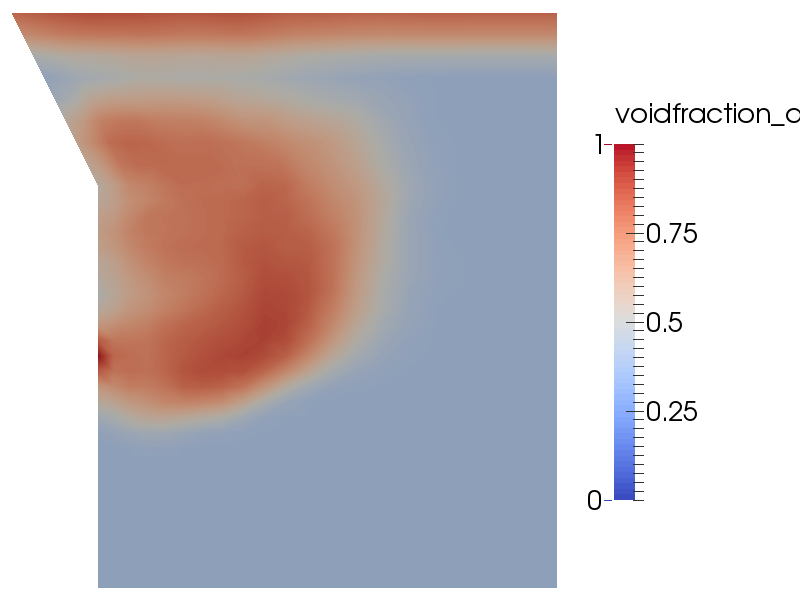
\includegraphics[width=.3\columnwidth]{images/253vf_average_lfhv}
	  \label{fig:253vf_average_lfhv}
  }
  \quad
    \subfloat[\acs{mus} = 0.9, \acs{mur} = 0.8, $v_{inlet}$ = 100 m/s .]
    {
	  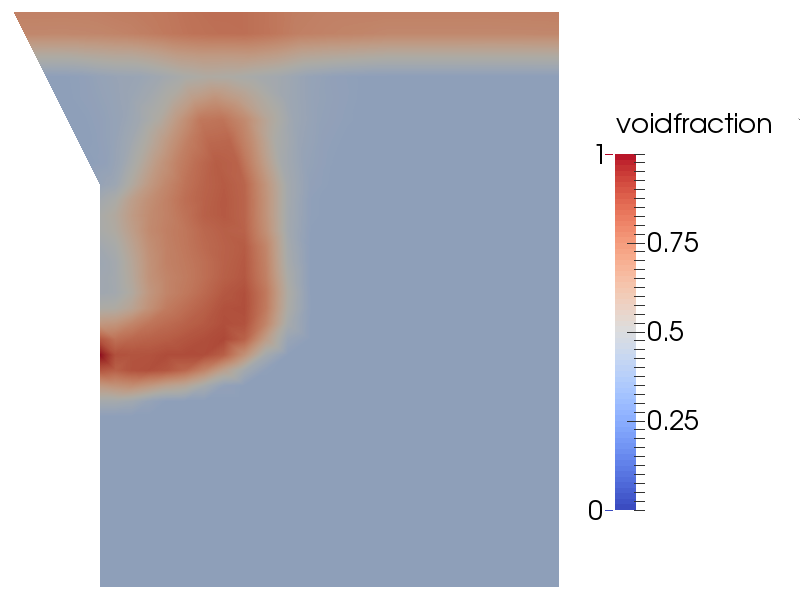
\includegraphics[width=.3\columnwidth]{images/252vf_average_hfhr}
	  \label{fig:252vf_average_hfhr}  }
  \\
  \caption{Average void fraction with different sliding friction coefficient.}
  \label{fig:239racewayvf}
\end{sidewaysfigure}